\documentclass{article}
\usepackage[a4paper, margin=1in]{geometry}
\usepackage{graphicx}

\title{Informação Profissional em Ciência da Computação:\\
	Seminário Arquitetura de Computadores}
\author{
    Carlos Eduardo Gallo Filho \\
	Caio Uehara Martins \\
	Pedro}
\date{\today}

\begin{document}
	\maketitle
	\graphicspath{ {./images/} }

	\section{Introdução}
		\subsection{Arquitetura x Organização}
		\subsection{Estrutura x função}
		\subsection{Estrutura single core x multi core}
		\subsection{Estrutura interna do core}
	\section{Breve história dos computadores: Primeira geração}
		\begin{flushleft}
			\qquad A primeira geração de computadores é conhecida pelo uso das válvulas para representar os elementos lógicos digitais e a memória. E também, o  	\textit{conceito de programa armazenado}, atribuída ao matemático John Von Neumann, que surgiu para a construção do computador EDVAC (Eletronic Discrete Variable Computer), mas foi principalmente discutido no desenvolvimento do computador IAS, o qual é um protótipo para quase todos os computadores de propósito geral de hoje em dia. 
		\end{flushleft}

		\subsection{Arquitetura de Von Neumann}
			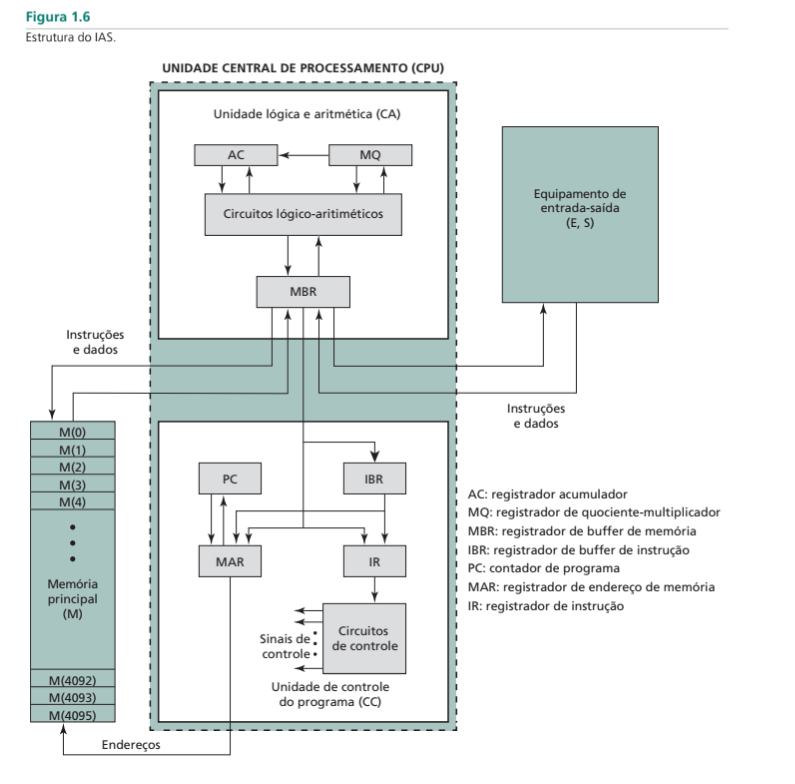
\includegraphics[scale=1]{estruturaDoIAS.jpg}	
		\subsection{Descrição dos elementos de Von Neumann}
			\begin{flushleft}
				~ \qquad Para explicar-se a estrutura do IAS, deve-se atentar a 5 partes principais. \\
 				\qquad 1) Um computador terá de ser capaz de executar as operações elementares básicas (adição, subtração, multiplicação, divisão). Normalmente, para essas funções são criadas unidades específicas para tais, comportadas em uma unidade maior centralizadora denominada CA ou unidade lógica e aritmética. \\
				\qquad 2) Um computador terá de ser capaz de dar sequenciamento adequado as suas operações, instruções e as instruções de controle (comandos que regem o próprio sequenciamento do computador). Á essas undides é denomiada uma unidade central chamada CC ou controle central. \\

				~ \qquad As partes 1) e 2) juntas são chamadas de C. \\

 				\qquad 3) Um computador terá a necessidade de processar sequências longas de operações, que, geralmente, não conseguem ser efetuadas em uma única leva de comandos. Logo, requer-se uma unidade que armazene dados por períodos duráveis para resolver problemas mais complexos, como cálculos.
Essa unidade é denominada M ou memória. \\

				~ \qquad Analogamente ao funcionamento do corpo humano, essas três partes podem ser comparadas a parte cognitiva do corpo. Ou seja, a unidade lógica e aritmética, o controle central e a memória são o conjunto pensante do computador. Mas, assim como o corpo humano, se faz necessário a comunicação com o mundo externo, tal é feito por um canal denominado meio de gravação de sáida do dispositivo ou R, de modo que as últimas duas partes interagem com esse canal para satisfazer a necessidade de interação com o externo. \\

				\qquad 4) A parte de entrada do meio R, a qual deve transferir as informações desse para dentro de M e C é chamada de entrada ou I. É de boa prática a entrada passar os dados para dentro de M e nunca diretamenta para C. \\
		
				\qquad 5) 	Similarmente, a parte de saída do meio R, a qual deve transferir as informações de M e C para o meio R, é chamada de saída ou O. É de boa prática, também, a saída passar de M para R, assim, nunca diretamente por C. \\

				~ \qquad Assim, resumidamente, temos a memória principal, que armazena dados e instruções; a unidade lógica e aritmética (ALU), que opera os binários; a unidade de controle, que interpreta e executa instruções e, por fim, o equipmaneto de saída (E/S), que conecta o meio interno ao meio externo do computador.

			
			\end{flushleft}
		\subsection{Endereçamento de memória}
	\section{Breve história dos computadores: Segunda geração}
	\section{Breve história dos computadores: Terceira geração}
	\section{Breve história dos computadores: Gerações posteriores}
\end{document}